\chapter{Introduction}\label{C:intro}

Time series contain valuable insights about the underlying system that generates the data. 
Their analysis is typically conducted using two primary approaches: time-domain and transformed-domain methods. 
In the context of time-domain analysis, Bandt and Pompe \cite{PhysRevLett.88.174102} introduced a novel methodology that is non-parametric and rooted in information theory descriptors: Ordinal Patterns symbolization. 

Bandt and Pompe \cite{PhysRevLett.88.174102} proposed transforming small subsets of the time series observations into symbols that encode the sorting properties of the values in these subsets.
Then, they computed a histogram of those symbols.
The resulting distribution is less sensitive to outliers compared to the original data, and the histogram is independent of any specific model.
The proposal proceeds by computing descriptors from this histogram, and extracting information about the system from these descriptors.
As a result, this approach is versatile and applicable to a wide range of scenarios.  

%%% ACF What do you mean by "This study"? If it is your thesis, is this what you do?
%%% ACF This paragraph is very misleading
%This study explores features derived from Bandt and Pompe symbolization, specifically Shannon entropy, complexity, and represents them graphically in the entropy-complexity plane, which is represented as a point in the $\mathbb{R}^2$ manifold. 
%%% ACF Is the Shannon Entropy a point in the HxC plane?
%%% ACF Is that true under the Multinomial distribution?
The proposal focuses on the statistical properties of features from ordinal patterns in time series clustering. It involves calculating pattern histograms, entropy, complexity, and confidence intervals to better understand the statistical properties of these tools. 
Additionally, the role of confidence intervals in entropy and complexity, along with their applications in time-series clustering, will be explored. Future work will expand to include alternative measures, such as Rényi entropy, Tsallis entropy and Fisher information, with a focus on deriving confidence intervals for their entropy and complexity under the Multinomial model. 

Time series analysis is widely applied across various fields, including engineering, economics, physical sciences, and more. A time series is defined as a collection of observations ${x_t}$, each representing a realized value of a particular random variable $X_t$, where time can be either discrete or continuous.

Examples of time series applications include finance (e.g., analyzing exchange rate movements or commodity prices), biology (e.g., modeling the growth and decline of bacterial populations), medicine (e.g., tracking the spread of diseases like COVID-19 or influenza), and geoscience (e.g., predicting wet or dry days based on past weather conditions).

The primary goal of time series analysis is to understand the nature of the phenomenon represented by the observed sequence. Time domain and frequency domain methods are the two primary approaches used in time series analysis. The temporal approach relies on concepts such as auto-correlation and regressions, where a time series' present value is analyzed in relation to its own past values or the past values of other series. This method represents time series directly as a function of time. On the other hand, the spectral approach represents time series through spectral expansions, such as wavelets or Fourier modes~\cite{treitel1995spectral}.


However, these methods often require assumptions such as large sample sizes or normally distributed observations that are rarely met in real-world empirical data. For many statistical techniques to be valid, these assumptions must hold, but in practice, they are frequently violated.

For example, traditional approaches to time series analysis, such as time domain and frequency domain methods, rely on assumptions that are not always valid in real-world data. The time domain approach, which uses techniques like auto-correlation and regression, assumes stationary and often struggles with nonlinear or non-stationary data. Similarly, the frequency domain approach, which represents time series through spectral expansions such as wavelets or Fourier modes, may require assumptions about periodicity and may not effectively capture short-term fluctuations.

Many statistical methods in these approaches depend on specific conditions, such as large sample sizes or normally distributed observations. However, these assumptions are often unrealistic, leading to inaccurate or biased results. When such conditions are not met, alternative methods must be considered.

%%% ACF Do you use the KW test again? You have defined H as the notation for its statistics, while H becomes entropy
As a result, alternative methods, commonly known as non-parametric techniques, are often considered. These approaches do not rely on the actual numerical values of the observations $x_t$, but rather on their ranks $R_t$, making them more robust and less sensitive to outliers and applicable to a wide range of data sets. 
%For examples, the Mann–Whitney U test, Spearman’s rank correlation, Wilcoxon test are effective tools for comparing two or more population probability distributions from independent random samples. 
Since non-parametric tests do not assume any specific distribution, such as normality, they are considered highly reliable for a range of data types.

However, while these techniques are powerful for general statistical analysis, they are not always well-suited for time series data. 

To address these challenges, ordinal pattern methods provide a robust alternative. Instead of analyzing the absolute values of a time series, these methods focus on the order relationships among consecutive data points.

This approach effectively captures the underlying dynamics of complex systems and offers several advantages.

The ordinal pattern-based method has become a widely used tool for characterizing complex time series. Since its introduction nearly twenty-three years ago by Bandt and Pompe in their foundational paper \cite{PhysRevLett.88.174102}, it has been successfully applied across various scientific fields, including biomedical signal processing, optical chaos, hydrology, geophysics, econophysics, engineering, and biometrics. It has also been used in the characterization of pseudo-random number generators.

The Bandt and Pompe method successfully analyzes time series by transforming them into ordinal patterns, constructing a histogram, and computing Shannon entropy, making it robust against outliers and independent of predefined models.


\section{Introduction to Ordinal Pattern Analysis}

%%% ACF Is this a good sentence? Read it out loud
Ordinal patterns are a non-parametric representation of real-valued time series by transforming small subsets of observations into symbols based on their relative order, rather than looking into actual values. This approach maps each segment of the time series in $\mathbb{R}^D$ into a finite set of $D!$ distinct symbols, where $D$ represents for the ''Embedding Dimension'' and usually ranges between three to six. 
One of the possible encoding is the set of indexes that sort the $D$ values in non-decreasing order.

To illustrate this idea, let $\bm{x}=\{x_1,x_2, \dots, x_{n+D-1}\}$ 
be a real valued time series of length $n+D-1$ without ties. 
The corresponding symbol sequence naturally emerges from the time series without requiring any model assumptions. We compute
$\bm{{\pi}}=({\pi}_1, {\pi}_2,\dots, {\pi}_n)$ symbols from sub-sequences of embedding dimension $D$. 
There are $D!$ possible symbols: $\pi_j \in \{{\pi}^1, {\pi}^2,\dots, {\pi}^{D!}\}$, for each $1\leq j\leq n$.
%%% ACF Revise the following sentence; it is unclear
The histogram of proportions $h=(h_1,h_2,\dots, h_{D!})$ in which the bin $h_\ell$ 
is the proportion of symbols of type $\pi^\ell$ of the total number of symbols. 
For convenience, we will model those symbols as a $k$ dimensional random vector where $k=D!$.

%%% ACF Do you need this here?
%%% ACF Be careful: the multinomial model requires independent trials. When you tranform a time series into symblos, there is no independence
%%Consider a series of $n$ independent trials in which only one of $k$ mutually exclusive events ${\pi}^1, {\pi}^2,\dots, {\pi}^k$ is observed with probability $p_1, p_2, \dots, p_k,$ respectively, where $p_\ell \geq 0$ and $\sum_{\ell=1}^{k} p_\ell=1$. 
%%Suppose that $N=(N_1, N_2, \dots, N_k)$ is the vector of random variables that, with $\sum_{\ell=1}^{k} N_\ell=n$, counts how many times the events ${\pi}^1, {\pi}^2,\dots, {\pi}^k$ occur in the $n$ trials. Then, the joint probability distribution of $N$ is
%%% ACF NEVER leave a blank line between the paragraph and the equation that follows
%%\begin{equation}
%	\Pr\big(N=(n_1,n_2,\dots, n_k)\big) = n! \prod_{\ell=1}^{k} \frac{p_\ell^{n_\ell}}{n_\ell !}, %%% ACF Propagate the changes
%%\end{equation}    
%where $n_\ell \geq 0$ and $\sum_{\ell=1}^{k} n_\ell=n$ .


\section{Problem Statement}

To illustrate this concept, imagine tracking the mean monthly humidity in Wellington. You want to analyze how humidity changes throughout the year. By examining this data, you can uncover interesting patterns that highlight the variations in humidity across different months. 

\begin{table}[hbt]
	\centering
	\begin{tabular}{lc}
		\toprule
		Month & Mean of relative humidity \\
		\midrule
		January & 77.3 \\ 
		February & 81.0 \\
		March & 82.4 \\
		April & 81.7 \\
		May & 83.6 \\ 
		June & 85.6 \\
		July & 84.4 \\
		August & 83.1 \\ 
		September & 78.8 \\
		October & 79.6 \\
		November & 78.2 \\
		December & 78.8 \\
		\bottomrule
	\end{tabular}
	\caption{Mean monthly humidity variations in Wellington throughout the year}
	\label{tab:humidity}
\end{table}

The mean monthly humidity in Wellington is shown in Figure~\ref{fig:humidity}.

\begin{figure}[hbt]
	\centering
	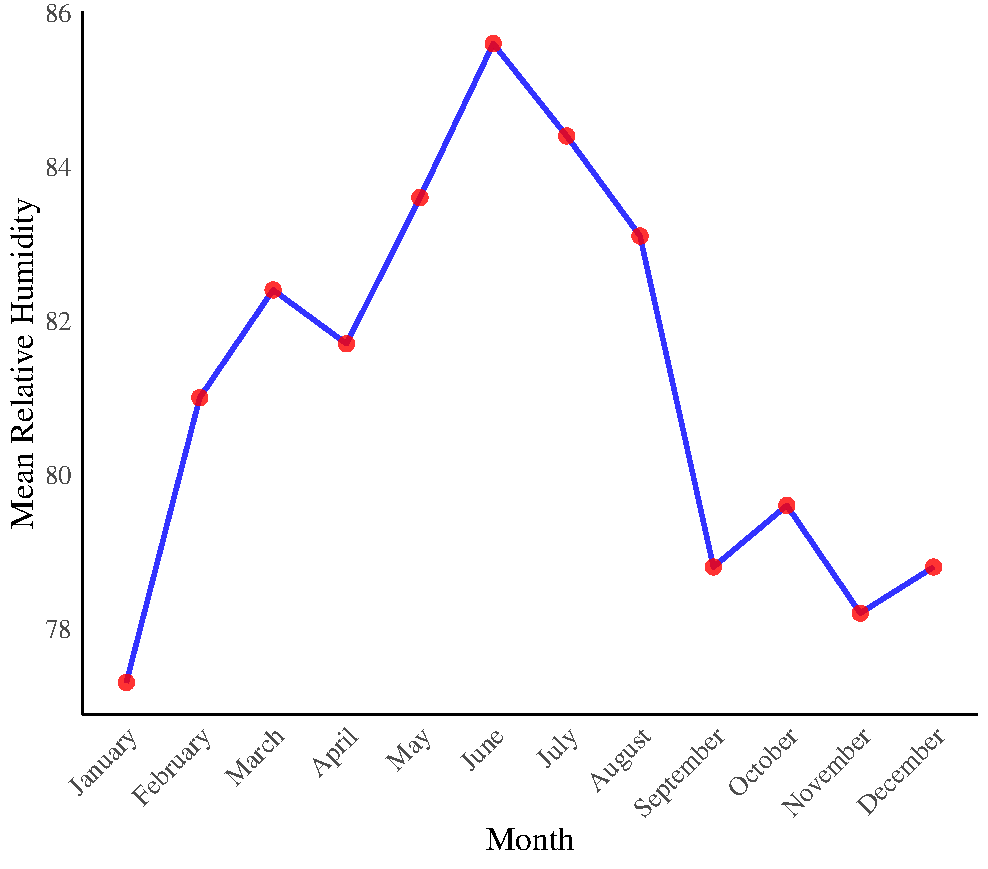
\includegraphics[width=0.6\textwidth]{humidity graph}
	\caption{Mean Monthly humidity in Wellington}
	\label{fig:humidity}
\end{figure}

We can convert this actual data into ordinal patterns. 
To do this, for each month, we determine the order of the humidity values rather than their actual magnitudes. 
Each three-time-point sequence (which can be adjusted based on preference) is converted into an ordinal pattern.
This ``embedding dimension'' usually varies between $3$ and $6$, but any dimension is possible.
The conversion can be made in any way that uniquely maps the sorting properties of the sub sequence into a symbol.
For example, consider the time series presented in Table \ref{tab:humidity}. We can transform this series into ordinal patterns as follows. 
%%% ACF You haven't defined the time lag. You won't use the time lag is this example. Do you you need it at this point?
Assume we use patterns of length $D=3$. 
The first overlapping window $(77.3,81,82.4)$ corresponds to the pattern  $(1,2,3)$, where type is considering with the order of the real time series data. Here $77.3$ is the smallest value and is assigned rank $1$; $81$ is the next highest and is assigned rank $2$; and $82.4$ is the largest, assigned rank $3$. As another example, consider the overlapping window $(83.1, 78.8, 79.6)$.  In this case, $78.8$ is the smallest value and is assigned rank $1$; $79.6$ is the next highest, assigned rank $2$; and $83.1$ is the largest, assigned rank $3$. Therefore, the pattern for this window is $(3,1,2)$.
Table \ref{tab:op} has shown this scenario. 
%%% ACF Summarise and present in your own words from Section 3
%@Article\{AsymptoticDistributionofEntropiesandFisherInformationMeasureofOrdinalPatternswithApplicationsa,
%author    = \{Rey, A. A. and Frery, A. C. and Gambini, J. and Lucini, M.\},
%journal   = \{Chaos, Solitons \textbackslash{}\& Fractals\},
%title     = \{Asymptotic distribution of entropies and \{F\}isher information measure of ordinal patterns with applications\},
%year      = \{2024\},
%issn      = \{0960-0779\},
%month     = nov,
%pages     = \{115481\},
%volume    = \{188\},
%doi       = \{10.1016/j.chaos.2024.115481\},
%groups    = \{Journal Article\},
%publisher = \{Elsevier BV\},
%\}


%%% ACF Use only the lines provided by the booktabs package
%%% ACF The table is confusing: "# of patterns" should be just $t$, Ordinal Patters should be Ordinal pattern, and you should assign a type to each, i.e., \pi^1, \pi^2 etc

\begin{table}[H]
	\centering
	\begin{tabular}{lcr}
		\toprule
		$t$ & Mean Humidity sequence & Ordinal Pattern \\
		\midrule
		1 & (77.3,81,82.4) & (123) $=\pi^1$\\ 
		2 & (81,82.4,81.7) & (132) $=\pi^2$\\
		3 & (82.4,81.7,83.6) & (213) $=\pi^3$\\
		4 & (81.7,83.6,85.6) & (123) $=\pi^1$ \\
		5 & (83.6,85.6,84.4) & (132) $=\pi^2$\\ 
		6 & (85.6,84.4,83.1) & (321) $=\pi^6$\\
		7 & (84.4,83.1,78.8) & (321) $=\pi^6$\\
		8 & (83.1,78.8,79.6) & (312) $=\pi^5$\\ 
		9 & (78.8,79.6,78.2) & (231) $=\pi^4$\\
		10 & (79.6,78.2,78.8) & (312) $=\pi^5$\\
		\bottomrule
	\end{tabular}
	\caption{Ordinal Patterns}
	\label{tab:op}
\end{table}

As shown in Table~\ref{tab:op}, we have six mutually exclusive events which we denote as   
$\{{\pi}^1, {\pi}^2,\dots, {\pi}^{6}\}= \{(123),(132),(213),(231),(312),(321)\}$. 
The probability distribution of the mean humidity is calculated based on ordinal patterns as given below.
\begin{equation}
	\hat{p_i}=\frac{\#\{\pi_j \in \bm{\pi}: \pi_j=\pi^{i}\}}{n}; 1\le i \le 6,
\end{equation}
where $\hat{\bm{p}}=(\hat{p_1}, \dots ,\hat{p_6})$.

\begin{table}[hbt]
	\centering
	\begin{tabular}{lc}
		\toprule
		Notation & Probability \\ 
		\midrule
		$p(\pi^1)$ & $\frac{2}{10}$ \\ 
		$p(\pi^2)$ & $\frac{2}{10}$ \\
		$p(\pi^3)$ & $\frac{1}{10}$ \\
		$p(\pi^4)$ & $\frac{1}{10}$ \\
		$p(\pi^5)$ & $\frac{2}{10}$ \\ 
		$p(\pi^6)$ & $\frac{2}{10}$ \\
		\bottomrule
	\end{tabular}
	\caption{Probability function}
	\label{tab:probability_function}
\end{table}

We construct the histogram of proportions $h=(h_1,h_2,h_3,h_4,h_5,h_6)$, where each bin $h_\ell$ represents the proportion of symbols of type $\pi^\ell$ out of the total six symbols. The histogram graph is shown Figure~\ref{fig:histogram}.

\begin{figure}[hbt]
	\centering
	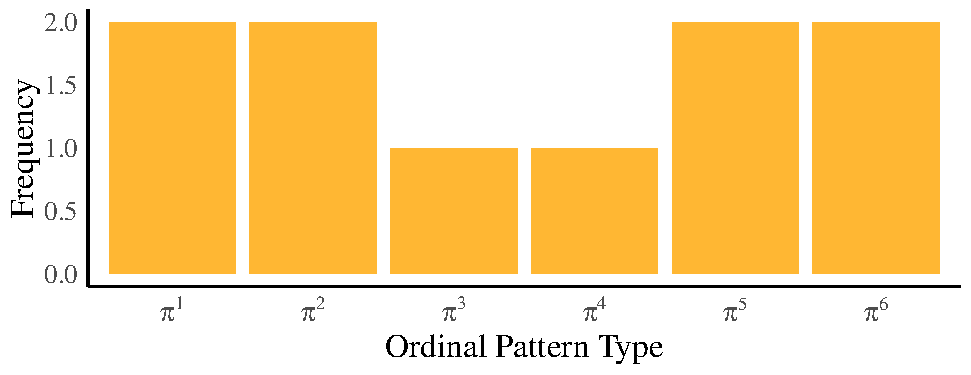
\includegraphics[width=0.6\textwidth]{frequency histogram}
	\caption{Histogram of proportions of the observed patterns according to Table~\ref{tab:probability_function}.}
	\label{fig:histogram}
\end{figure}
%%% ACF Always add information as in the following line
%%% The above plot was produced by lines 41-57 of file 'Code/R/humidity_example.R'

This example explains how time series data can be converted into ordinal patterns and how the probability distribution function can be calculated from these patterns.
%%% ACF The example should proceed by discussing, defining, and illustrating the permutation entropy and the statistical complexity
%%% ACF Do not be redundant
%% I didn’t address this comment because I swapped the chapters to improve the flow.
Chapter~\ref{C:aim} will expand on this concept by exploring the characterization of time series and cover the computation of two key descriptors entropy and complexity from the resulting histograms. Chapter~\ref{C:lit} will review the literature on ordinal pattern analysis. Additionally, Chapter~\ref{C:futw} will outline the main ideas and objectives of this research project.      






